\chapter{REVISÃO DA LITERATURA}
\thispagestyle{empty}

\section{Projetos}

  \citeonline[p. 8]{meredith2011project} definem que projetos tratam da realização de tarefas específicas e finitas, de grande ou pequena escala, com um prazo de execução e um orçamento estipulado. \citeonline{turner2014handbook}, por sua vez, dispõe que projetos são tarefas com uma data final, onde caso esta data não implique na entrega do projeto, será estabelecida uma entrega do produto presente e a criação de outro projeto para entregar as tarefas restantes, referente a este produto.

  Para \citeonline{kerzner2013project} um projeto pode ser caracterizado por uma série de atividades e tarefas realizadas com um objetivo específico para serem completadas sob determinadas especificações. Essas atividades e tarefas também devem possuir datas definida para inicio e fim; limites de recursos e custos; bem como um quantitativo de pessoas e equipamentos que será envolvido nestas.

  Finalmente, de acordo com o \citeonline{pmiguide2013}, um projeto pode ser compreendido por um esforço temporário empreendido a fim de criar um produto, prestar serviço ou trazer um resultado exclusivo. Esse esforço é composto por um conjunto de atividades inter relacionadas e direcionadas à obtenção de um ou mais produtos únicos, com tempo e custos definidos. Nesta definição, algumas características básicas do projeto devem ser destacadas:

  \begin{itemize}
    \item{\textbf{Delimitação temporal:} datas específicas para início e fim;}
    \item{\textbf{Objetivos:} metas definidas em função de um problema, oportunidade ou interesse da organização;}
    \item{\textbf{Elaboração progressiva:} etapas contínuas de desenvolvimento e incrementos;}
    \item{\textbf{Incerteza:} a representação do degrau entre o resultado esperado e as condições de realização do projeto;}
    \item{\textbf{Singularidade:} a representação da exclusividade do projeto, aquilo que o torna único;}
    \item{\textbf{Relação fornecedor-beneficiário:} relação entre quem desenvolve e quem recebe o projeto.}
  \end{itemize}

  Assim, pode-se compreender que todo projeto é essencialmente temporário e único, ou ainda, finito e regular, que frequentemente é utilizado, direta ou indiretamente, para alcançar os objetivos de um plano estratégico que, por sua vez, visa o desenvolvimento de um novo produto ou um serviço exclusivo.

\section{Gestão de Projetos}

  De acordo com \citeonline[p. 74]{kerzner2013project} a gestão de projetos pode ser considerada uma metodologia que consiste em um processo repetitivo usado em projetos com o objetivo de alcançar sua maturidade. Afirma-se também que qualquer metodologia, inclusive a mais simples, pode representar um caso de sucesso como prática de GP, desde que seja aceita na organização em questão. Entretanto, ao utilizar uma metodologia de GP de sucesso, a probabilidade de que a organização se destaque como entregadora de bons projetos será elevada \cite{kerzner2013project}.

  Para \citeonline{pmiguide2013}, a GP implica no uso de ferramentas, técnicas e da competência de utilizar recursos como: o conhecimento de conceitos, características próprias e particulares, bem como fatores críticos de sucesso para o aprimoramento e entrega de projetos de excelência. Destaca-se ainda como características importantes, porém não exclusivas:

  \begin{itemize}
    \item Identificação dos requisitos;
    \item Abordagem das diferentes necessidades, preocupações e expectativas das partes interessadas no planejamento e execução do projeto;
    \item Estabelecimento, manutenção e execução de comunicações ativas, eficazes e colaborativas entre as partes interessadas;
    \item Gerenciamento das partes interessadas visando o atendimento aos requisitos do projeto e a criação das suas entregas;
    \item Equilíbrio das restrições conflitantes do projeto que incluem: [1] Escopo, [2] Qualidade, [3] Cronograma, [4] Orçamento, [5] Recursos, e [6] Riscos.
  \end{itemize}

  Essas características se mostram de suma importância e devem deter a devida atenção da equipe gerencial, pois podem influenciar nas restrições a serem estabelecidas nos projetos.

  Alguns autores afirmam que a garantia de que os objetivos definidos de projeto serão alcançados depende de um processo disciplinado, por parte da GP, que respeite custos, prazos e desempenho requeridos e que ocorra através do envolvimento de pessoas em atividades de planejamento e controle numa organização \cite{dinsmore2009ama, meredith2011project}.

\section{Associações de Gestão de Projetos}

  Considerando a importância dos processos empregados na GP, atualmente, existem alguns conjuntos de modelos oferecidos por determinadas organizações, formadas por profissionais, que servem de guia para melhor gerir projetos. Abaixo, no quadro~\ref{quadro_institutos}, estam ilustradas algumas das principais organizações e os modelos de referência oferecido por elas.

  \begin{quadro}[!h]
    \centering
    \caption{Principais associações de Gestão de Projetos \\ Fonte: Adaptação de \citeonline{patah2012metodos} \label{quadro_institutos}}
    \begin{tabular}{| m{.40\textwidth} m{.30\textwidth} m{.20\textwidth}|}
      \hline
      \textbf{Institutos} & \textbf{Conjunto de Métodos} & \textbf{País de Origem} \\
      \hline \hline
      \textit{Project Management Institute} (PMI) & \textit{Project Management Body of Knowledge} (PMBoK) & EUA \\ \hline
      \textit{International Project Management Association} (IPMA) & IPMA \textit{Competence Baseline} & União Européia \\ \hline
      \textit{Association for Project Management} (APM) & APM \textit{Body of Knowledge} & Reino Unido \\ \hline
    \end{tabular}
  \end{quadro}

  O quadro~\ref{quadro_referencias} serve de ilustração resumida dos principais pontos e diferencias dos modelos de referência citados anteriormente.

  \begin{quadro}[!h]
    \centering
    \caption{Modelos de referência de GP e suas principais caracteríticas. \\ Fonte: Adaptação de \citeonline{patah2012metodos} \label{quadro_referencias}}
    \begin{tabular}{| m{.20\textwidth} m{.40\textwidth} m{.30\textwidth}|}
      \hline
      \textbf{Modelos} & \textbf{Caracteríticas} & \textbf{Diferencial} \\
      \hline \hline
      PMBoK – \textit{Project Management Body of Knowledg}
        & Por ser desenvolvido para diversos tipos de projetos é considerado bastante genérico. Sua estrutura é composta pelas áreas de conhecimento de um projeto.
        & É complementado por dois conjuntos de métodos: Programa e Portfólio. \\ \hline
      IPMA \textit{Competence Baseline}
        & Sua estrutura é composta pelas competências que os projetos necessitam para se desenvolver, isto é, contexto; comportamento; e técnicas.
        & Apresenta um alto grau de profundidade nos aspectos humanos e na figura do gerente do projeto. \\ \hline
      APM \textit{Body of Knowledge}
        & Apresenta um conteúdo vasto relacionado a projetos, valor, escritório de projetos e aspectos estratégicos da gestão de projetos.
        & Pode ser considerado o mais completo e abragente modelo. \\ \hline
    \end{tabular}
  \end{quadro}

  A seguir será apresentado um breve contexto sobre estas instituições e seus modelos.

  \subsection{Project Management Institute (PMI)}

    O PMI foi fundado em 1969, como uma instituição sem fins lucrativos, que se baseou na premissa de que existiam muitas práticas comuns de GP em diversas áreas de projetos, entre elas, nas áreas de contrução e de produção farmaceútica \cite{pmiguide2013}. Atualmente esse instituto é conhecido por disseminar o conhecimento sobre GP em diversos paises, mais de 160 paises com aproximadamente 540.000 membros, sendo sua sede situada nos Estados Unidos (EUA), conforme ilustrado no Quadro~\ref{quadro_institutos} \cite{pmi2013}.

    Em \citeonline{prado2004gerenciamento} afirmam considerar o PMI como principal instituição mundial responsável pelo reconhecimento e padronização das ações relacionadas a GP. Entre suas principais publicações encontra-se o ``PMBOK - Project Managemant Body of Knowledge'', ou como foi traduzido em português ``Um Guia do Conjunto de Conhecimentos em Gerenciamento de Projetos''.

    Atualmente, em sua 5a edição, é possivel observar que o PMBoK é um conjunto de boas práticas, consideravelmente genérico e abragente, que visa atender às necessidades de diversas áreas e portando de muitos tipos de projetos \cite{pmiguide2013}.

    Ele se encontra dividido em 47 processos de GP, sendo estes subdivididos em dez áreas de conhecimento: [1] Integração; [2] Escopo; [3] Tempo; [4] Custos; [5] Qualidade; [6] Recursos Humanos; [7] Riscos; [8] Comunicação; [9] Aquisições; [10] Partes Interessadas, e em cinco grupos de processos:

    \begin{itemize}
      \item \textbf{Iniciação:} processos executados para definir um novo projeto ou nova fase de um projeto;
      \item \textbf{Planejamento:} processos necessários à elaboração do Plano de Gerenciamento do Projeto, que define as ações necessárias para alcançar seus objetivos;
      \item \textbf{Execução:} processos realizados para executar o trabalho definido no Plano de Gerenciamento do Projeto;
      \item \textbf{Monitoramento e Controle:} processos exigidos para acompanhar, analisar e controlar o progresso e desempenho do projeto;
      \item \textbf{Encerramento:} processos necessários para finalizar todas as atividades do projeto, visando encerrar formalmente o projeto.
    \end{itemize}

    A Figura~\ref{processos_areas_pmbok} representa a divisão da relação das àreas de conhecimento pelos grupos de processos do PMBoK.

    \begin{figure}[!h]
      \centering
      \scalebox{0.3}{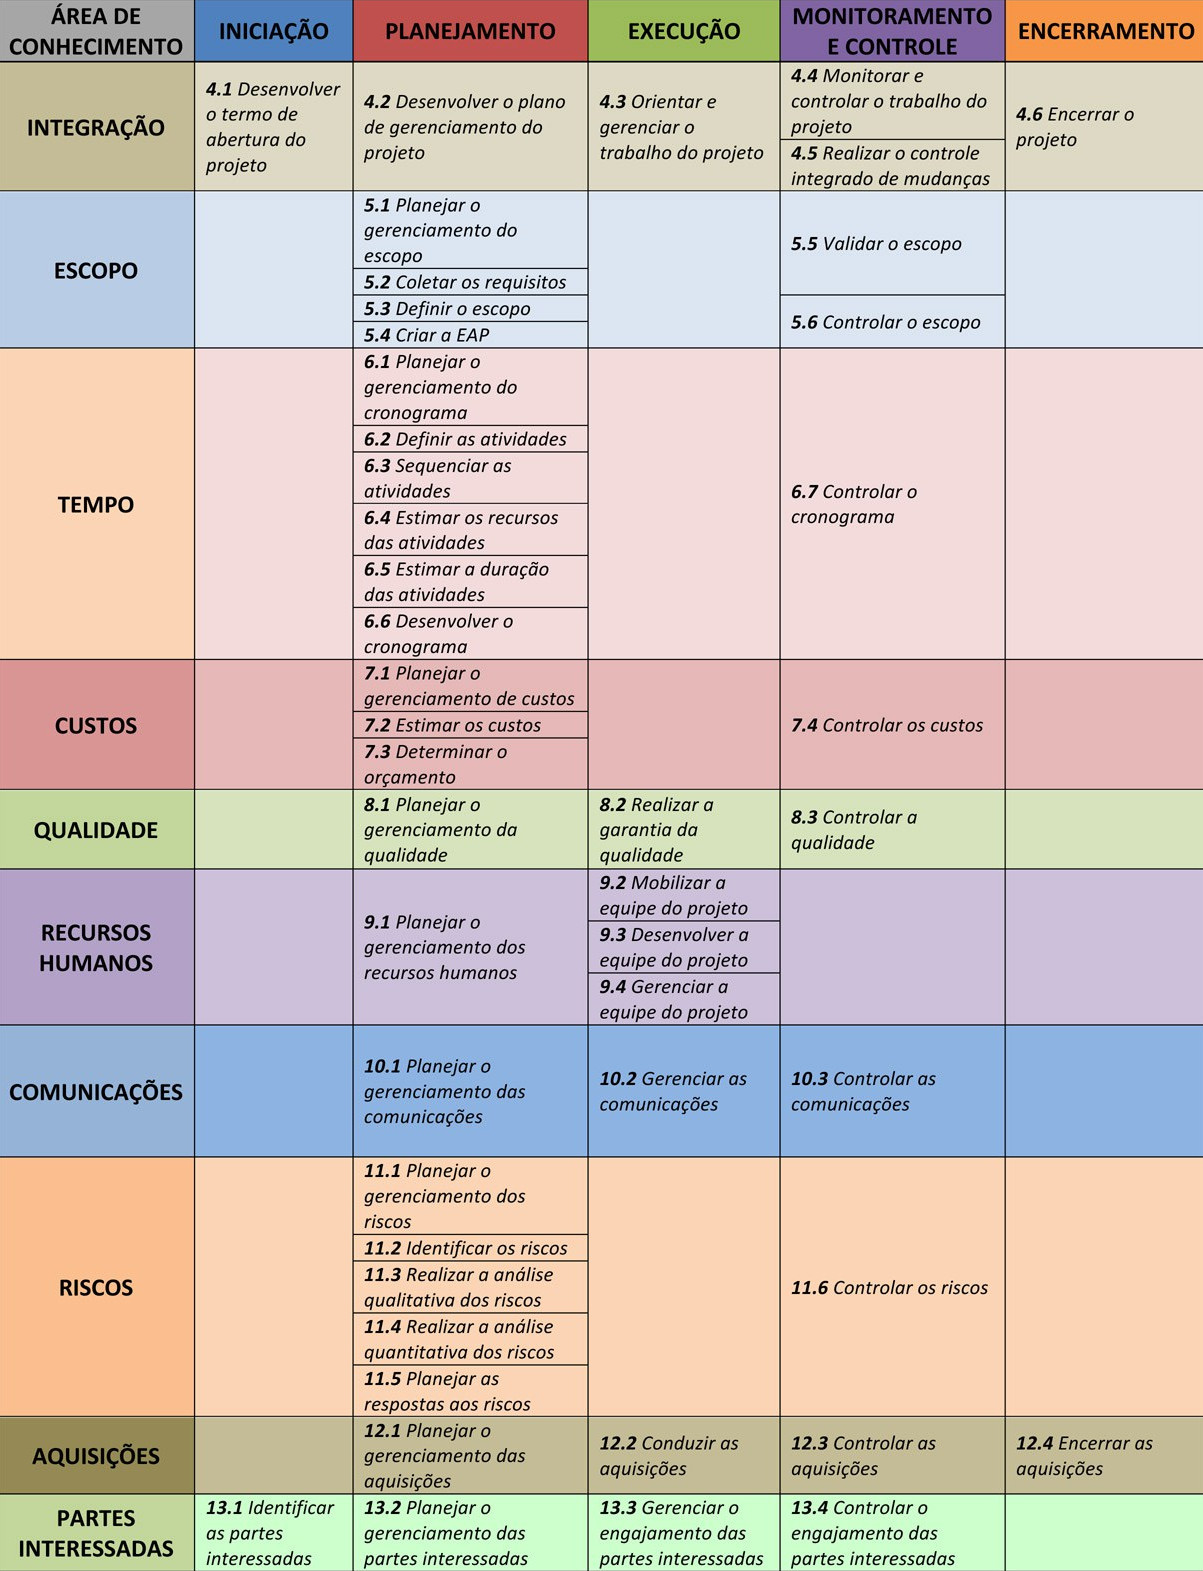
\includegraphics{figuras/processos_areas_pmbok}}
      \caption{Relação dos grupos de processos pelas àreas de conhecimento. Fonte: \cite{pmiguide2013}}
      \label{processos_areas_pmbok}
    \end{figure}

  \subsection{International Project Management Association (IPMA)}
  \subsection{Association for Project Management (APM)}

\section{Gestão de Programas}

  Programas podem ser entendidos por estruturas que consistem em uma equipe principal e um conjunto de equipes de projeto que averiguam capacidade de decisão e autoridade de um membro definitivo, isto é, um gerente de programa que assegura a direção e as decisões desta estrutura. Estas estruturas visam alcançar um determinado objetivo dentro de uma estratégia.\cite{brown2008handbook}.

  \citeonline{rijke20141197} avalia que apesar da dificuldade geral em distinguir um programa de um projeto, a gestão de programas deve ser considerada mais extensa que gestão de projetos, pois ela abrange áreas em que projetos singulares não se encontram. Vale ressaltar também que o gestor de programa tem hábitos mais estratégicos que podem interferir na GP \cite{lycett2004289}.

  Assim, a gestão de programas tem sido cada vez mais adotada por organizações com o objetivo de implementar estratégias que integrem melhor seus projetos e ferramentas, sem permitir que o desempenho possa desorientar a natureza estratégica das decisões.

\section{Gestão de Portfólio}

  A gestão de portfólio, conhecida também por Gestão de Portfólio de Projetos (GPP), surgiu a partir da necessidade de gerenciar investimentos em projetos nas organizações. Seu processo dinâmico e integrado visa avaliar o alinhamento estratégico e a viabilidade da execução simultânea de diversos projetos ao mesmo tempo. Esses projetos passam por uma introspecção que os seleciona e organiza de acordo com sua priorização em um portfólio \cite{meredith2011project, kerzner2013project}.

  De acordo com \citeonline[p. 27]{burke2013project}, um portfólio pode abrigar conjuntos de projetos, programas e até mesmo outros portfólios que não precisam estar diretamente relacionados, mas que se reúnem por uma questão de otimização e controle. A Figura~\ref{port_prog_proj} ilustra a relação entre portfólio, programas e projetos.

  \begin{figure}[!h]
    \centering
    \scalebox{0.4}{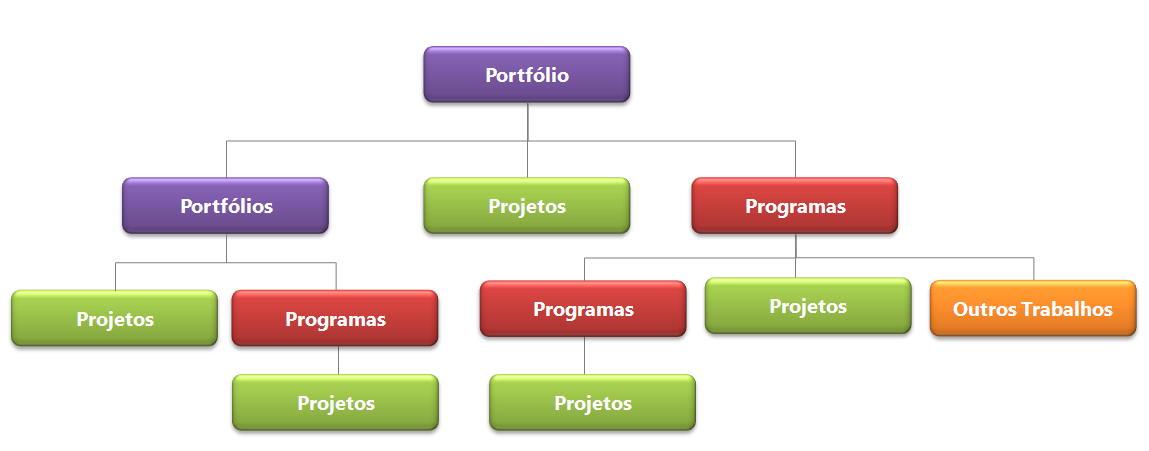
\includegraphics{figuras/port-prog-proj}}
    \caption{Relação Portfólio, Programas e Projetos. Fonte: \cite{pmi2006}}
    \label{port_prog_proj}
  \end{figure}

  \citeonline[p 11]{pmiguide2013} estabelece que o critério de agrupamento de um portfólio deve visar a facilitação na gestão para que seja possível atingir os objetivos estratégicos de uma organização. É definido ainda que toda gestão de portfólio fique sob responsabilidade de um EGP. A figura \ref{estrategia_portfolio} representa os processos incorporados pela Gestão de Portfólio.

  \begin{figure}[!h]
    \centering
    \scalebox{0.4}{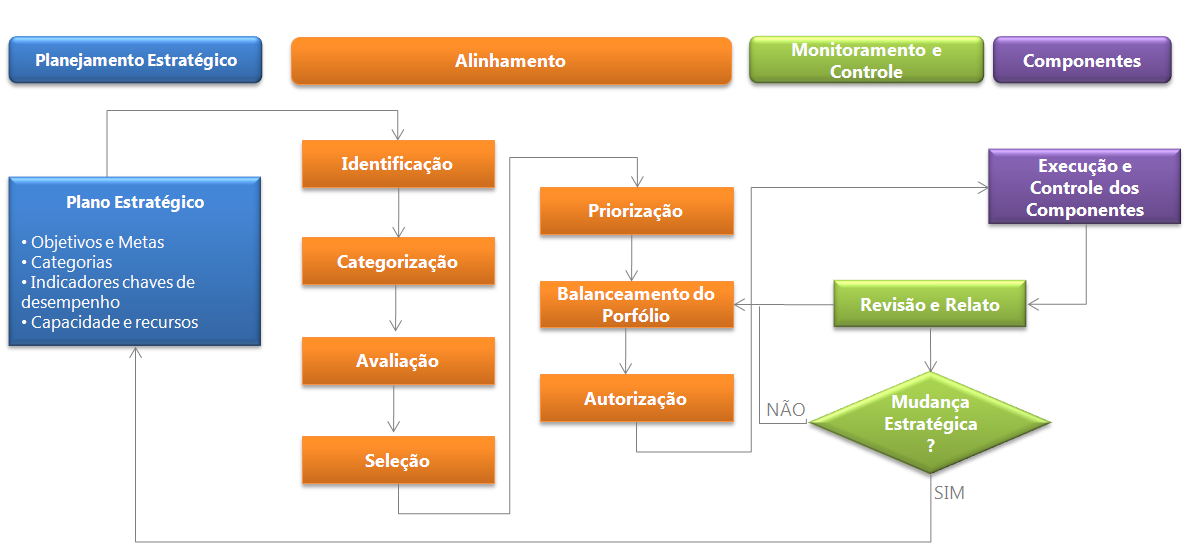
\includegraphics{figuras/estrategia-portfolio}}
    \caption{Processos de Gestão de Portfólio. Fonte: \cite{pmi2006}}
    \label{estrategia_portfolio}
  \end{figure}

  Desta forma, a GPP pode ser dita como uma manifestação de estratégia de negócios que determina os investimentos da organização via processos simultâneos, sistemáticos e dinâmicos de decisão, tornando o sucesso do EGP dependente do desempenho agregado de iniciativas dos componentes do portfólio e buscando a maximização do uso e do alinhamento desses componentes \cite{pmiguide2013}.

\section{Escritorio de Gestão de Projetos}

  Advindo do inglês \textit{Project Management Office}(PMO), o escritório de gestão de projetos (EGP), ou ainda escritório de projetos (EP), pode ser considerado um conjunto de profissionais de GP que servem a um modelo organizacional com o propósito de aumentar a eficiência e lidar com as necessidades da GP, assumindo um papel de alta confiança ao implementar diversas estratégias em projetos \cite{kendall2003advanced}.

  Através de um estudo, \citeonline{pemsel2013project} identificou três principais atividades que são esperadas do EGP:

  \begin{itemize}
    \item Promover e facilitar o desenvolvimento estratégico da GP, bem como o uso estratégico de objetos que sejam empreendidos na GP;
    \item Planejar, controlar e dar suporte a GP, sempre assegurando que o conhecimento seja compartilhado no processo para melhorar sua eficiência;
    \item Adoção estratégias de treinamento, negociação e formação para prover o desenvolvimento de competências.
  \end{itemize}

  Para \citeonline{dinsmore2005pmo} a principal expectativa empregada por um EGP esta relacionada ao suporte e orientação; ao processo de desenvolvimento e gerenciamento de projetos mais eficiente e eficaz o possível; e ao uso de metodologias e recursos de planejamento e análise de projetos padronizadas.

  De acordo com \citeonline{crawford2010strategic}, por mais simples que um EGP possa ser, suas atividades compõem estruturas complexas responsáveis por atividades de planejamento, controle e monitoramento, cuja implantação representa um processo de mudança de cultura organizacional, por estar diretamente relacionada à negociação com pessoas. O autor retrata ainda três níveis de atuação do EGP que podem ser visualizados na Figura~\ref{pmo_crawford}.

  \begin{figure}[ht]
    \centering
    \scalebox{0.6}{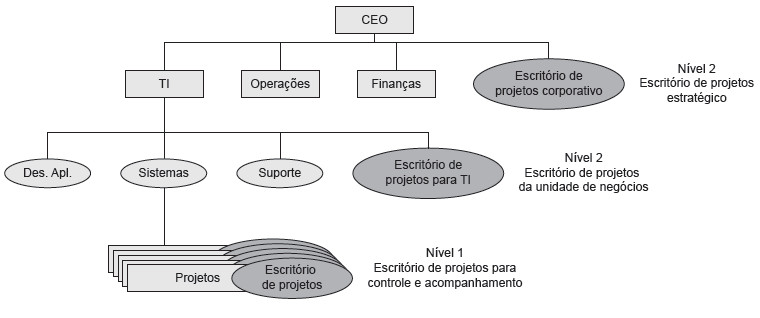
\includegraphics{figuras/pmo-crawford}}
    \caption{Níveis de atuação do escritório de projetos. Fonte: \cite{crawford2010strategic}.}
    \label{pmo_crawford}
  \end{figure}

  As competências desses níveis podem ser representas como \cite{crawford2010strategic}:

  \begin{itemize}
    \item \textbf{Nível 1 - Escritório de Controle de Projetos:} visa o desenvolvimento do planejamento de projetos individualmente, realizando também a emissão de relatórios de progresso. Embora tenha foco em apenas um projeto, geralmente este projetos apresenta grande porte e complexidade;
    \item \textbf{Nível 2 - Escritório de Projetos da Unidade de Negócios:} oferece suporte a todos os projetos de uma área específica, porém de porte e complexidade variados;
    \item \textbf{Nível 3 - Escritório Estratégico de Projetos:} possui as seguintes competências:
    \begin{itemize}
      \item Selecionar, priorizar e garantir a integração de cada projeto para que esteja alinhado à estratégia da organização, inclusive no que respeito aos seus recursos;
      \item Desenvolver, atualizar e divulgar a metodologia de GP bem como seus conhecimentos;
      \item Converte-se em centro da gestão de conhecimento da organização através do armazenamento de informações sobre lições aprendidas;
      \item Validar estimativas de recursos realizadas pelo projetos, baseando-se em experiências anteriores.
    \end{itemize}
  \end{itemize}

  Assim, as responsabilidades de um EGP podem variar de acordo com a centralização empregada na organização, uma vez que está relacionada a padronização dos processos de GP. Entretanto as ferramentas e técnicas a serem empregadas ficam sob critério do gestor responsável pelo EGP \cite{pmiguide2013}.

  Alguns autores, ainda, apontam o EGP como uma ferramenta de apoio para que organizações obtenham bom desempenho em GP, bom como para alcançarem seus objetivos estratégicos. Esses mesmos autores destacam que fatores comuns ligados as taxas de sucesso do EGP, em caso positivo, devem ser enfatizados, enquanto em caso negativos, devem ser evitados, configurando assim boas práticas para o sucesso do EGP \cite{andersen2007benchmarking}.

\section{Sistemas de Gestão de Projeto}

  Ao contrário do que é esperado pela natureza de negócios ou operações usuais, a natureza dos projetos e serviços é representada por processos curtos, repetitivos e funcionais, que facilitam a identificação de padrões usualmente inseridos em soluções de informação. Assim, especialista de GP veem o uso de sistemas de gestão de produtos (SGP), como uma ferramenta preciosa no que respeito a alcanço os objetivos e na excelência de projetos \cite{cserban2011project}.

  Seguindo mais além, \citeonline{prado2006mmgp} afirma que diversos aspectos das metologias de GP dependem indiretamente do uso de SGP, sem que porém, seja determinada a natureza do SGP. O autor infere ainda que só é possível para organizações almejarem determinados níveis de maturidade se utilizarem essas ferramentas.

  Através de um estudo quantitativo, \citeonline{liberatore2001project} analisou que nunca antes a adoção de uma ferramenta para auxiliar nas práticas de GP foi tão explorada quanto o uso de SGP. Os especialistas de GP demonstraram grande interesse pela facilidade encontrada no compreendimento da complexidade do projeto através desses sistemas, e expressaram interesse em integrar cada vez funcionalidades referente aos projetos.

  Por meio de uma revisão na literatura \citeonline{hartmann2009implementing}, acrescentou que além de auxiliar no tratamento da complexidade nos projetos, o uso de SGP também se destaca para o aprimoramento da produtividade do processo de projeto, apesar de também ser notada uma dificuldade inicial para o adaptamento do uso dessas ferramentas.

  Além de prover um meio para lidar com a produtividade de processo e complexidade do projeto, já foi comprovado também que o uso de SGP influi nos processos de planejamento, comunicação, monitoramento, controle de riscos, cronograma, gerenciamento de documentos e ainda avaliação de custos \cite{raymond2008project}.

  Portanto, o uso de SGP implica em deter ferramentas capazes de facilitar e otimizar o esforço empregado pela GP para alcançar a excelência na realização do projeto, não apenas por parte do uso dos gestores do projeto, mas também por incluir outros atores presentes em seus processos \cite{cserban2011project}.

\section{Maturidade em Gestão de Projetos}

  Maturidade pode ser compreendida por uma qualidade ou por um estado de amadurecimento. Se aplicado a uma organização, o conceito de maturidade estaria diretamente relacionado com a sua capacidade de entregar produtos ou serviços em perfeitas condições para que seus objetivos sejam alcançados.

  Para \citeonline{kerzner2006projeto} maturidade consiste no desenvolvimento de sistemas e processos de natureza repetitiva que vêem a garantir uma alta probalidade de sucesso. Esses processos podem ser dividos em níveis de capacidade que estabelecem o quanto uma empresa se aprimorou, e o quanto é preciso de incrementos para que a mesma melhore seu desempenho.

  Quando relacionada a GP, a maturidade tende a ilustrar o grau em que uma organização realiza procedimentos ligados a GP em suas atividades, viabilizando sua expansão e crescimento. Esse grau é definido de acordo com a utilização de boas práticas referenciadas em um modelo de maturidade \cite{fahrenkrog2003project}.

  Os modelos de maturidade de GP representam uma abordagem quantitativa que parte da premissa que organizações evoluem por meio de processos contínuos de desenvolvimento e crescimento, e que tais processo permitem aferir práticas e atividades frente a uma estrutura progressiva. Espera-se ainda que esses modelos representem o caminho a ser seguido pela organização para gerir necessidades dinâmicas, como a falta de capacitação dos recursos humanos, ou a necessidade de conciliar atrasos e orçamentos que se mostram inviáveis, entre outros \cite{de2013fatores}.

  Para \citeonline{pmiguide2013} a maturidade em GP simboliza pelo nível de habilidade de uma organização na entrega de resultados estratégicos desejados, que sejam ainda previsíveis, controláveis e confiáveis. Compreende-se então que o nível de maturidade de uma empresa está diretamente relacionado a sua capacidade de obter sucesso em seus projetos, onde ter sucesso significa entregar o projeto dentro do escopo, prazo, custo e qualidade planejada.

  De acordo com o relatório anual \citeonline{pmsurvey2015}, no Brasil, os modelos de maturidade mais utilizados são o \textit{Organizational Project Management Maturity Model} (OPM3), proposto pelo PMI, e o Modelo de Maturidade em Gerenciamento de Projetos (MMGP), proposto por Prado e Archibald.

  \subsubsection{Capability Maturity Model (CMM)}

    O \textit{Capability Maturity Model} (CMM) foi um dos primeiros modelos de maturidade lançados e reconhecidos. Desenvolvido na Universidade Carnegie Mellon, com parceria com de \textit{System Engineering Institute}, visou auxiliar o departamento de defesa americano a escolher fornecedores de software, tomando como base atitudes gerenciais de empresas de desenvolvimento de software \cite{carvalho2011fundamentos}.

    \begin{figure}[!h]
      \centering
      \scalebox{0.6}{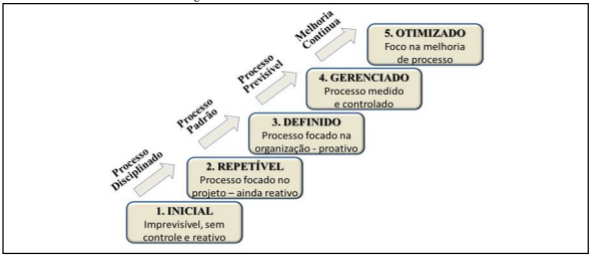
\includegraphics{figuras/cmm}}
      \caption{Níveis de maturidade do modelo CMM.\\ Fonte: Adaptado de \cite{mezzena2007beneficios}.}
      \label{cmm}
    \end{figure}

    A Figura~\ref{cmm} reproduz os cinco níveis de maturidade previstos no modelo CMM. Logo abaixo, encontra-se uma breve descrição da principal característica de cada nível, que correspondem a um conjunto de áreas chaves de processo \cite{mezzena2007beneficios} :

    \begin{itemize}
      \item \textbf{Nível 1 – Inicial:} caracteriza-se pela informalidade do processo de desenvolvimento de software, caótico e com ações reativas, frequentemente ultrapassando os prazos e custos dos projetos;
      \item \textbf{Nível 2 – Repetível:} possui os processos básicos de GP para o acompanhamento de cronograma, custos e funcionalidades já implantados, permitindo repetir sucessos anteriores;
      \item \textbf{Nível 3 – Definido:} existe um processo integrado padrão para a organização, em que os procedimentos de GP e atividades de engenharia estão documentados e são utilizados de forma padronizada;
      \item \textbf{Nível 4 – Gerenciado:} utiliza-se medições detalhadas de processos de desenvolvimento e qualidade de produtos, que são analisados e controlados de forma quantitativa;
      \item \textbf{Nível 5 – Otimizado:} obtem a implantação de um processo de melhoria contínua, por meio da retroalimentação quantitativa e análises comparativas, na busca de novas ideias e tecnologias inovadoras.
    \end{itemize}

  \subsubsection{Project Managenet Maturity Model (PMMM)}

    Proposto por \citeonline{kerzner2006projeto}, o modelo \textit{Project Managenet Maturity Model} (PMMM) propõe cinco níveis de maturidade para que uma organização possa alcançar a excelência de GP, na Figura~\ref{pmmm}, é possível observar esses níveis:

    \begin{figure}[!h]
      \centering
      \scalebox{0.6}{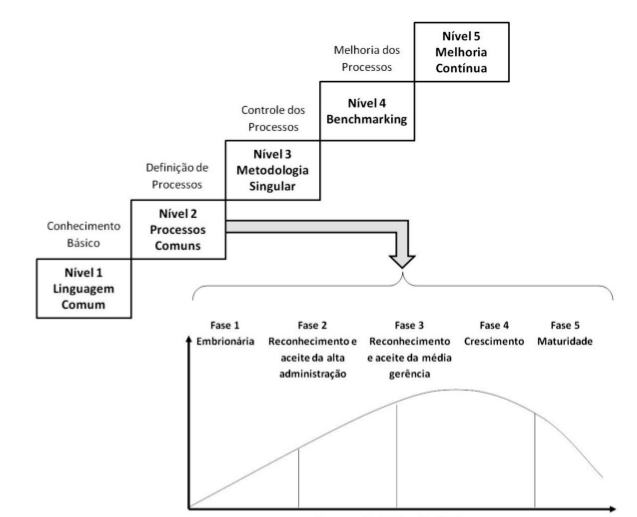
\includegraphics{figuras/pmmm}}
      \caption{Os cinco níveis da Maturidade PMMM.\\ Fonte: Adaptado de \cite{kerzner2006projeto}.}
      \label{pmmm}
    \end{figure}

    Basicamente, cada nível pode ser exemplificado em:

    \begin{itemize}
      \item \textbf{Nível 1:} a organização reconhece a importância da GP e a necessidade de um conhecimento básico nas atividades a ela relacionadas;
      \item \textbf{Nível 2:} a organização verifica a necessidade de processos comuns, utilizados em todos os projetos;
      \item \textbf{Nível 3:} a organização se conscientiza dos ganhos que a combinação entre a metodologia de GP e outras práticas utilizadas pela empresa podem trazer;
      \item \textbf{Nível 4:} a organização reconhece que um processo de melhoria é necessário para manter as vantagens competitivas;
      \item \textbf{Nível 5:} a organização analisa as informações obtidas através da comparação e decide se essas informações trarão benefícios.
    \end{itemize}

    O autor \citeonline{crawford2007project} aponta o nivel 2, ``processos comuns'', como um nível determinante. Isto é, antes de atingir este nível, a organização esta relativamente desorganizada quanto aos processos de GP, porém, após atingí-lo, a organização passará a compreender melhor seus processos e a necessidade de melhorias.

  \subsubsection{Organizational Project Management Maturity Model (OPM3)}

    O modelo \textit{Organizational Project Management Maturity Model} (OPM3) foi proposto em 2003 pelo PMI, como um modelo de maturidade genérico, cujo principal propósito se traduz em auxiliar organizações a desenvolver a capacidade de controlar e melhorar os processos de seus projetos. Ele inclui ainda um método de avaliação e melhoria sistemática que pode ser utilizado, tanto separadamente em cada projeto, quanto aplicado a um portfólio \cite{berssaneti2012impact}

    De acordo com \citeonline{lianying2012project}, em sua primeira versão, o OPM3 contava apenas com um questionário de avaliação geral do projeto, enquanto em 2008, em sua segunda versão, passou a contar com critérios que avaliassem também a organização, quanto aos meios estruturais, culturais, tecnológicos e de recursos humanos. Levando também em consideração o novo conceito PMI de portfólio.

    Finalmente, em 2013, foi lançada a edição atual do modelo, juntamente com a atualização mais recento do conjunto de boas práticas PMBoK. Além de se alinhar com a versão atual do PMBoK, esta edição incluiu também critérios acordados com os livros \textit{The Standard of Program Management} e \textit{The Standard for Portfolio Management}, que tratam respectivamente sobre gestão de programas e de GPP \cite{pmiopm2013}

    O modelo possui ferramentas e métodos que possibilitam a identificão de problemas e deficiências, bem como a realização de diagnósticos e avaliação contínua dos projetos visando a implementação de melhorias. Sua documentação em formato de livro, dispõe de informações explicativas e necessárias para GP, além de uma relação de melhores práticas e um meio para avaliar o real estado dos projeto \cite{fahrenkrog2003project}

    Através dos critérios de avaliação do OPM3, foram definidos quatros estágios de desenvolvimento para cada nível de maturidade \cite{pmiopm2013}:

    \begin{itemize}
      \item \textbf{Padronização:} identifica o processo-problema;
      \item \textbf{Aferição:} identifica as entradas/saídas; priorizar e definir indicadores;
      \item \textbf{Controle:} identifica os indicadores e variações, e analisa as causas raízes;
      \item \textbf{Melhoria contínua: } identifica e implementa mudanças nos processos.
    \end{itemize}

    A Figura~\ref{pmbok_opm3} ilustra a relação dos grupos de processos do PMBoK pelos níves de maturidade do OPM3:

    \begin{figure}[!h]
      \centering
      \scalebox{0.8}{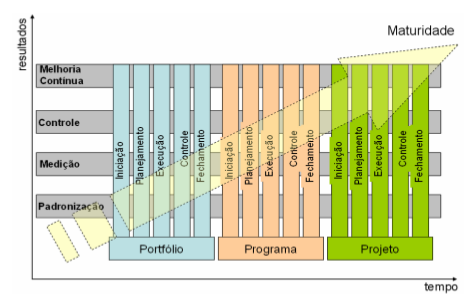
\includegraphics{figuras/pmbok-opm3}}
      \caption{Relação dos grupos de processos PMBOK pelos níves de maturidade do OPM3. \\ Fonte: Adaptado de \cite{pmiopm2013}}
      \label{pmbok_opm3}
    \end{figure}

    Assim, tendo como paramêtro a importância do PMI como instituição disseminadora de conhecimentos de GP, e a compatibilidade do modelo de maturidade OPM3, sugere-se que este seja o modelo de melhor aceitação pelos profissionais de GP.

  \subsubsection{Modelo de Maturidade em Gerenciamento de Projetos}

    % \begin{figure}[!h]
    %   \centering
    %   \scalebox{0.6}{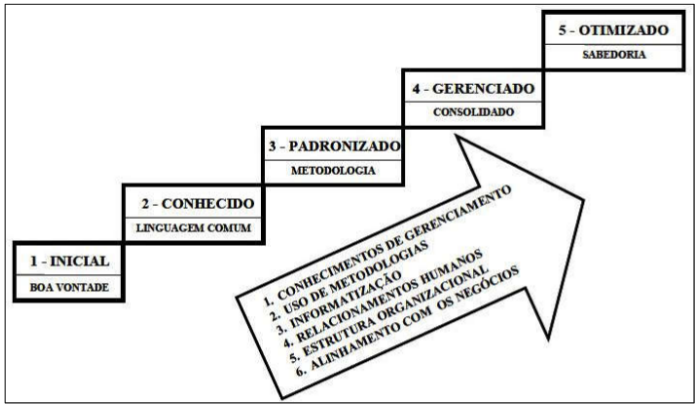
\includegraphics{figuras/mmgp}}
    %   \caption{Dimensões e níveis de maturidade do modelo Prado - MMGP.\\ Fonte: Prado e Archibald (2006, p.131).??? \cite{kerzner2006projeto}.}
    %   \label{mmgp}
    % \end{figure}

\section{Fatores Críticos de Sucesso}
% > conceito sucesso
% Sucesso em Gestão de Projetos é frequentemente definido como a conclusão do projeto com atendimento da totalidade do escopo dentro do prazo e custo planejados e com a qualidade esperada. No entanto, existem variações deste entendimento.
% Shenhar, Levy e Dvir (1997 apud NORO; BONZATTI, 2013, p. 86) afirmam que as pessoas possuem diferentes percepções em relação ao conceito de sucesso, e que essa percepção varia no tempo.
% Kerzner (2006, p. 41-42) afirma que “o problema de definir sucesso como a concretização do prazo programado, dentro do orçamento e com níveis de qualidade desejado é que todos estes indicadores constituem uma definição interna de sucesso”. Segundo o autor o sucesso é definido pelo cliente. “Pode-se concluir um projeto internamente no prazo, no orçamento e nos limites de qualidade para só então descobrir que o cliente não gostou dos resultados.”

% Vargas (2003, p. 18) afirma que “um projeto bem-sucedido é aquele que é realizado conforme planejado”. Como a maioria dos autores, Vargas (2003, p. 19) considera que o sucesso de um projeto pode ser medido pela obtenção dos resultados esperados, dentro do prazo, custo e qualidade desejados. Porém, ressalta que outros parâmetros são importantes. O autor define os seguintes critérios para considerar um projeto como bem-sucedido:
% - Ser concluído dentro do tempo previsto;
% - Ser concluído dentro do orçamento previsto;
% - Ter utilizado recursos (materiais, equipamentos e pessoas) eficientemente, sem desperdícios;
% - Ter atingido a qualidade e a performance desejada;
% - Ter sido concluído com o mínimo possível de alteração de seu escopo;
% - Ter sido aceito sem restrições pelo contratante ou cliente;
% - Ter sido empreendido sem que ocorresse interrupção ou prejuízo nas atividades normais da organização;
% - Não ter agredido a cultura da organização.

% Prado e Archibald (2015) classificam os projetos em três categorias quanto ao sucesso:
% Sucesso total: Um projeto bem-sucedido é aquele que atingiu a meta. Isto geralmente significa que foi concluído e produziu os resultados e benefícios esperados e os principais envolvidos ficaram plenamente satisfeitos. Além disso, mas não obrigatoriamente, espera-se que o projeto tenha sido encerrado dentro das exigências previstas para prazo, custo, escopo e qualidade (pequenas diferenças podem ser aceitas).
% Sucesso parcial ou comprometido: o projeto foi concluído, mas não produziu todos os resultados e benefícios esperados. Existe uma significativa insatisfação entre os principais envolvidos. Além disso, provavelmente algumas das exigências previstas para prazo, custo, escopo e qualidade foram significativamente excedidas.
% Fracasso: existe uma enorme insatisfação entre os principais envolvidos ou porque o projeto não foi concluído ou porque não atendeu às expectativas dos principais envolvidos ou porque algumas das exigências previstas para prazo, custo, escopo e qualidade foram excedidas de forma absolutamente inaceitável.

% Conforme o PMI (2015, p. 8) a pesquisa Pulse revelou em média o percentual de projetos bem sucedidos é de 64\%, sendo considerado como projeto bem-sucedido aquele que atinge seus objetivos. O PMI (2015, p. 5) acredita que até que mais organizações comecem a investir na compreensão do valor da GP, no desenvolvimento de talentos (capacitação) na padronização de processos, as taxas gerais de sucesso de projetos não irão melhorar.

% > fatores críticos de sucesso em GP

